\chapter{Fundamentul teoretic}
\label{chapter:background}

\section{Rolul algoritmilor de localizare a sursei unui semnal}
\label{sec:role-doa}
De-a lungul anilor, cerințele impuse asupra sistemelor de telcomunicații
wireless au crescut radical, devenind din ce în ce mai importantă eficiența lor
spectrală. Rețelele trebuie să facă față unui număr ridicat de utilizatori, unor
aplicații multimedia cu cerințe mari de date, menținând, în același timp, o
latență cât mai redusă. O tehnică deosebit de utilă care s-a impus pentru
satisfacerea acestor exigențe este tehnica accesului multiplu cu diviziune în
spațiu (SDMA), care permite alocarea aceluiași canal unor utilizatori din zone
diferite, putând astfel reutiliza canale în interiorul unei celule. \\
\abbrev{SDMA}{Space-Division Multiple Access}

Pe baza tehnicii SDMA s-au dezvoltat sisteme de antene inteligente, care se
folosesc de algoritmi de procesare a semnalelor pentru a-și optimizia
caracteristica de radiație în funcție de semnalele primite. Un rol important îl
au algoritmii de localizare a sursei unui semnal, pe baza cărora, folosind un
algoritm de beamforming adaptiv, antenele își ajustează amplitudinile și fazele
pentru a transmite în direcția utilizatorului dorit. Astfel, crește capacitatea
de acoperire în interiorul unei celule, iar sistemul este capabil să diferențieze
semnalele utile de cele nedorite, ceea ce duce și la creșterea capacității
sale.

% \todo{Poate asta merge mai bine la motivatie} \\
% \todo{Caut mai multe despre localization si la MS, asa as justifica de ce e
% necesar un procesor cu consum de putere redus and stuff. Plus ca ar trebui sa
% aflu niste date precise despre ConnexArray, gen de ce e atat de important si ce
% economisesc cu el, ca justificare.} \\
% \todo{About using directional reception check link below}
% %https://worldwide.espacenet.com/publicationDetails/biblio?CC=US&NR=5345599&KC=&FT=E&locale=en_EP
% %https://google.com/patents/WO2000051368A3?cl=no
% 
% 
% Antenele multiple atât la transmițător, cât și la stația mobilă sunt deja
% folosite în sistemele mobile 4G și se preconizează că ele vor sta și la baza
% noului standard 5G~\cite{5g-what-will-be}. \\

\section{Algoritmi de localizare a sursei unui semnal}
\label{sec:localization-algo}

Metodele folosite pentru estimarea direcției de incidență se clasifică, în
funcție de criteriul folosit, în metode convenționale, metode bazate pe
separarea subspațiilor zgomotului sau semnalului, metoda similitudinii maxime
etc. Din prima categorie fac parte Metoda convențională de Beamforming,
cunoscută și drept Metoda Bartlett, precum și Metoda Varianței Minime a lui
Capon, denumită și MVDR \abbrev{MVDR}{Minimum Variance Distortionless Response}.
Ce au în comun aceste metode este faptul că formează un fascicul convențional,
pe care îl scanează peste o anumită zonă, iar direcția care produce cea mai mare
putere de ieșire este considerată direcția de incidență~\cite{beamforming-doa}.
În practică, pentru metoda Bartlett, se scanează cu un anumit unghi $\theta$
aria dorită, obținându-se ca răspuns vectorul director $a(\theta)$. Pe baza
acestuia, se calculează matricea de covarianță $R_{xx}$ și puterea de ieșire se
calculează conform Ecuației~\eqref{eq:conv-power}.

\begin{equation}
\label{eq:conv-power}
    P(\theta) = \frac{a^H(\theta)R_{xx}a(\theta)}{a^H(\theta)a(\theta)}
\end{equation}

Se găsește direcția de incidență ca fiind unghiul corespunzător valorii maxime a
puterii de ieșire. Pentru a rezolva problemele de rezoluție slabă, se folosește
un filtru liniar cu anumite ponderi pentru a evita distorsionarea semnalului de
interes și se calculează, în schimb, inversa produsului dintre matricea de
covarianță și vectorul director~\cite{doa-smart-antenna}. \\

Metodele bazate pe separarea subspațiilor se folosesc de ortogonalitatea dintre
subspațiul format de semnalul de intrare și subspațiul format de zgomotul
suprapus peste acesta. Ele ating o rezoluție ridicată, dar cu cerințe mari de
procesare și de stocare și depind de o corelație cât mai slabă între semnalul de
intrare și zgomot. Dacă raportul semnal-zgomot este foarte scăzut, sau sursele
sunt foarte apropiate, performanțele acestor algoritmi se
deteriorează~\cite{subspace-performance}. Acestei categorii îi aparțin
algoritmii MUSIC \abbrev{MUSIC}{MUltiple SIgnal Classification} și ESPRIT
\abbrev{ESPRIT}{Estimation of Signal Parameters via Rotational Invariant
Techniques}. \\

În această lucrare, am analizat algoritmul MUSIC atât datorită performanțelor sale,
precum și modalității sale de analiză și estimare, care se pliază pe cerințele
actuale din domeniul comunicațiilor, ce vor fi detaliate în continuare.

\section{Algoritmul MUSIC}
\label{sec:theory-music}

\begin{figure}[h]
    \centering
    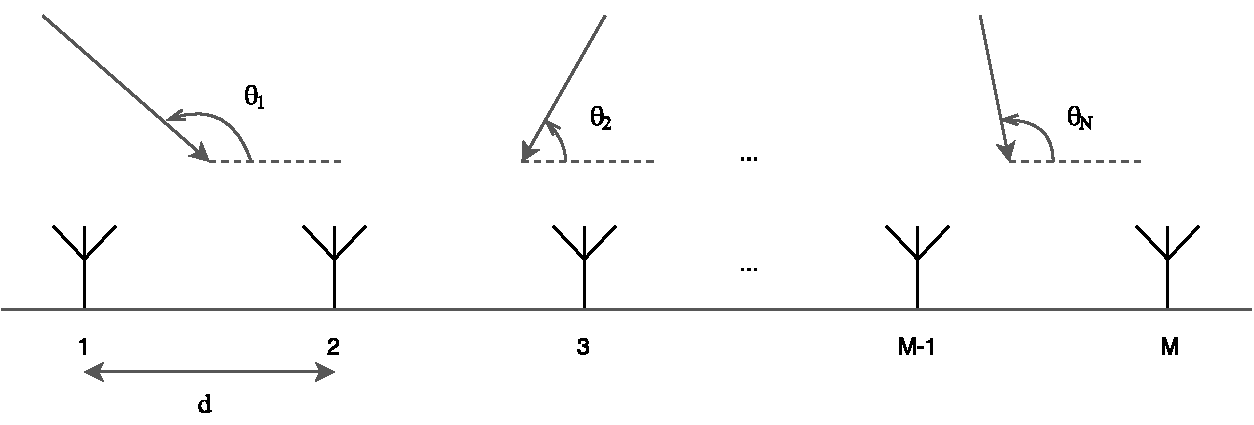
\includegraphics[width=1\textwidth]{src/img/signals}
    \caption{Configurația inițială în algoritmul MUSIC}
    \label{fig:array-for-doa}
\end{figure}


În analiza algoritmului MUSIC presupunem că plecăm de la un șir liniar de $M$
antene la care ajung $N$ semnale $s_j(t), i = \overline{1, N}$ și se dorește
estimarea unghiului de incidență $\theta_j$ măsurat față de axa $x$ în sens
trigonometric sub care ajunge fiecare semnal la șirul de antene, ca în Figura
\ref{fig:array-for-doa}. Pe parcursul lucrării, vom considera doar cazul unui
sistem liniar de antene, deci ne vom referi la el pur și simplu ca la un
,,sistem de antene'', fără a mai menționa caracterul său liniar. Presupunem că
mediul de propagare nu afectează semnificativ semnalele când acestea se propagă
de la un element din șir la altul, deci semnalul care ajunge la o antenă diferă
de cel care ajunge la o altă antenă doar printr-o întârziere $\tau$. \\

Considerăm că prima antenă se află în originea sistemului, la locația (0, 0) și
exprimăm întarzierea semnalului de la celelalte elemente din șir relativ la
semnalul care ajunge la elementul de referință. Astfel, pentru un șir liniar,
semnalul $j$ care ajunge la elementul $i = 2$ parcurge o distanță mai lungă cu
$d\,cos\theta_j$ față de primul element și, în cazul general, putem scrie
întârzierea $\tau_i$ la elementul $i$ ca
\begin{equation}
    \tau_i = \beta(i-1)d\,cos\theta_j
\end{equation}
unde $\beta = \frac{2\pi}{\lambda}$ este factorul de defazaj. \\

Aici, am presupus că defazajul semnalului depinde doar de locațiile distincte
ale elementelor șirului de antene. În realitate, antenele vor avea și ele un
răspuns dependent de directivitatea lor și de frecvență, care poate fi modelat
ca un câștig $g_i$. Obținem, astfel, vectorul director (\textit{steering
vector}) pentru un anumit unghi de incidență $\theta_j$ și frecvență $\omega$:
\begin{equation}
    \bm{a}(\omega, \theta_j) = 
	    \begin{bmatrix}
		g_1(\omega, \theta_j)e^{\tau_1(\theta_j)} \\
		... \\
		g_M(\omega, \theta_j)e^{\tau_M(\theta_j)}
	    \end{bmatrix}
\end{equation}

Prin urmare, vectorul director este dependent de răspunsul individual al
fiecărui element din șirul de antene, de geometria șirului, de frecvența
semnalului și de unghiul de incidență al acestuia. Matricea care se formează din
vectorii coloană directori pentru toate unghiurile de incidență și toate
frecvențele se numește matricea colectoare a șirului
(\textit{array manifold matrix}).
\begin{equation}
    \bm{A} = 
	    \begin{bmatrix}
		\bm{a}(\omega, \theta_1) & ... & \bm{a}(\omega, \theta_N)
	    \end{bmatrix}
\end{equation}

Dacă banda semnalului este suficient de îngustă, se poate considera, cu
aproximație, că vectorul director este independent de frecvență și că depinde doar
de unghiul de incidență. Mai mult, dacă presupunem că elementele șirului sunt
izotrope, putem elimina dependența vectorului director de câștigul $g_i,
i = \overline{1, M}$. Vom continua analiza având în vedere aceste presupuneri.\\

Putem scrie următoarea relație pentru semnalele de la intrarea fiecărei antene
din șir:
\begin{equation}
\label{eq:xasn}    
    \bm{x}(t) = 
	\begin{bmatrix}
	   \bm{a}(\theta_1) & \bm{a}(\theta_2) & ... & \bm{a}(\theta_N)
	\end{bmatrix}
	\begin{bmatrix}
	    s_1(t) \\ s_2(t) \\ ... \\ s_N(t)
	\end{bmatrix}
	+
	\begin{bmatrix}
	    n_1(t) \\ n_2(t) \\ ... \\ n_N(t)
	\end{bmatrix}
\end{equation}
\begin{equation}
\label{eq:xasn-short}
    \bm{x}(t) = \bm{A}\bm{s}(t) + \bm{n}(t)
\end{equation}

Algoritmul MUSIC (MUltiple SIgnal Classification)~\cite{music-schmidt} face
parte dintr-o clasă mai mare de algoritmi care se bazează pe metoda
subspațiilor, care ia în considerare și zgomotul dintr-un sistem. Algoritmul
oferă, în primul rând, informații despre numărul de semnale care ajung la un
șir de antene și unghiul de incidență al acestora. Este un algoritm cu
rezoluție mare, ceea ce înseamnă că poate distinge mai ușor decât alți
algoritmi două semnale care vin din direcții foarte apropiate, dar are nevoie
de o calibrare foarte precisă a șirului de antene.  Calibrarea constă în
obținerea matricei colectoare a șirului de antene; în practică, acest lucru se
realizează măsurând răspunsurilor unor surse punctiforme ale șirului la diverse
unghiuri și frecvențe. Pentru explicarea fundamentului matematic din spatele
algoritmului MUSIC s-a folosit ca referință lucrarea~\cite{doa-1996}, în care
este tratat pe larg subiectul estimării unghiurilor de incidență folosind
șiruri de antene.\\

În ecuația \eqref{eq:xasn}, vectorul $\bm{x}$ al semnalelor de la intrarea
antenelor din șir și vectorii directori $\bm{a}(\theta_j), j = \overline{1, N}$
pot fi priviți ca vectori într-un spațiu cu M dimensiuni, ceea ce înseamnă că
$\bm{x}$ poate fi scris ca o combinație liniară între vectorii directori, unde $s_j,
j = \overline{1, N}$ sunt coeficienții combinațiilor. \\

Se poate calcula matricea de covarianță a intrării
\begin{equation}
    \bm{R}_{xx} = E[\bm{xx}^H] = \bm{A}E[\bm{ss}^H]\bm{A}^H + E[\bm{nn}^H]
\end{equation}
\begin{equation}
    \bm{R}_{xx} = \bm{A}\bm{R}_{ss}\bm{A}^H + \sigma^2_{zg}\bm{I}
\end{equation}

S-a notat $\bm{R}_{ss} = E[\bm{ss}^H]$ matricea de corelație a semnalului $s$.
Se observă două proprietăți importante:
\begin{itemize}
    \item Vectorii directori sunt liniar independenți, ceea ce înseamnă că
    matricea $\bm{A}$ este de rang maxim.
    \item $\bm{R}_{ss}$ este o matrice nesingulară dacă semnalele incidente sunt
    cel mult parțial necorelate. Dacă ar fi corelate, atunci cel puțin una
    dintre liniile/coloanele sale ar putea fi scrisă ca o combinație liniară a
    altor linii/coloane, ceea ce ar însemna că matricea ar avea determinantul
    egal cu 0, deci ar fi singulară și nu am mai putea folosi algoritmul.
\end{itemize}

Din aceste două proprietăți rezultă că, dacă $M < N$, atunci matricea
$\bm{A}\bm{R}_{ss}\bm{A}^H$ este pozitiv semidefinită, având rangul N. Din
această proprietate, se poate demonstra faptul că $M - N$ dintre valorile
proprii ale matricei trebuie să fie nule. Folosind relația
\eqref{eq:xasn-short}, reiese că atunci când $M - N$ dintre valorile proprii ale
matricei $\bm{A}\bm{R}_{ss}\bm{A}^H$ sunt nule, cele mai mici valori proprii ale
matricei $\bm{R}_{xx}$ vor fi egale cu puterea zgomotului $\sigma_{zg}^2$. Dacă
notăm $\lambda_i, i = \overline{1, M}$ valorile proprii ale matricei
$\bm{R}_{xx}$, atunci
\begin{equation}
    \lambda_{N+1} = \lambda_{N+2} = ... = \lambda_M = \lambda_{min} = \sigma_{zg}^2
\end{equation}

În realitate, însă, nu se va îndeplini egalitatea, deoarece folosim
pentru estimare doar un număr finit de eșantioane, dar valorile vor fi,
într-adevăr, foarte apropiate. Dacă notăm $K$ multiplicitatea celei mai mici
valori proprii a matricei $\bm{R}_{xx}$, atunci, știind că $M = N + K$, putem
estima numărul semnalelor care ajung la șirul de antene
\begin{equation}
    \hat{N} = M - K
\end{equation}

Din definițiile valorilor proprii și a vectorilor proprii~\cite{gol-matrix}, vectorii
proprii $\bm{v}_i, i = \overline{1, M}$ corespunzători celor mai mici valori
proprii trebuie să satisfacă egalitatea
\begin{equation}
    \bm{R}_{xx}\bm{v}_i = \sigma_{zg}^2\bm{v}_i, \quad i = \overline{N+1, M}
\end{equation}
Folosind ecuația \eqref{eq:xasn-short}, înseamnă că
\begin{equation}
    \bm{A}\bm{R}_{ss}\bm{A}^H\bm{v}_i = 0, \quad i = \overline{N+1, M}
\end{equation}
Știind că $\bm{A}$ este de rang maxim și că $\bm{R}_{ss}$ este nesingulară,
atunci
\begin{equation}
    \bm{A}^H\bm{v}_i = 0, \quad i = \overline{N+1, M}
\end{equation}
ceea ce este echivalent cu a spune că vectorii coloană ai matricei $\bm{A}$,
adică vectorii directori, sunt perpendiculari pe vectorii proprii ai matricei
$\bm{R}_{xx}$. 
\begin{equation}
    \begin{bmatrix}
	\bm{a}(\theta_1) & \bm{a}(\theta_2) & ... & \bm{a}(\theta_N)
    \end{bmatrix}
    \bot
    \begin{bmatrix}
	\bm{v}_{N+1} & \bm{v}_{N+2} & ... & \bm{v}_M
    \end{bmatrix}
\end{equation}

Recapitulând, avem două subspații ortogonale: cel al semnalelor și cel al
zgomotului. Vectorii directori ai șirului de antene aparțin subspațiului
semnalelor și, așadar, sunt perpendiculari pe subspațiul zgomotului, iar
vectorii proprii ai matricei de covarianță $\bm{R}_{xx}$ pot aparține oricăruia
dintre cele două subspații. Prin urmare, putem să căutăm printre vectorii
directori pe aceia care sunt ortogonali pe subspațiul zgomotului, în care se vor
afla o parte din vectorii proprii ai matricei de covarianță, și să determinăm
unghiurile de incidență $\theta_j$.

Se calculează spectrul MUSIC folosind una dintre următoarele două forumle:
\begin{equation}
    P_{MUSIC}(\theta) =
        \frac{\bm{a}^H(\theta)\bm{a}(\theta)}
             {\bm{a}^H(\theta)\bm{V}_N\bm{V}_N^H\bm{a}(\theta)} \\
\end{equation}
\begin{equation}
    P_{MUSIC}(\theta) =
        \frac{1}
             {\bm{a}^H(\theta)\bm{V}_N\bm{V}_N^H\bm{a}(\theta)} \\
\label{eq:music-spectrum}
\end{equation}
\begin{equation}
    \bm{V}_N = \begin{bmatrix}v_{N+1}, & ..., & v_M \end{bmatrix}
\end{equation}
și, în cazul în care vectorii directori sunt perpendiculari pe vectorii proprii,
numitorul va fi minim, ceea ce va conduce la apariția unor vârfuri în spectru.
Cunoaștem numărul de semnale estimat $\hat{N}$, deci cele $\hat{N}$
vârfuri din spectru corespund unghiurilor de incidență căutate.

\section{Arhitectura Connex-ARM}
\label{sec:cnx-arr}

În această lucrare vor fi evaluate performanțele algoritmului studiat pe un
sistem cu arhitectura Connex-ARM~\cite{energy-effective-simd}, ce conține
elemente specifice atât paradigmei setului de instrucțiuni extins, cât și
paradigmei procesor gazdă-accelerator (\textit{host-accelerator paradigm}), și care este
implementat pe platforma Xilinx Zynq-7000~\cite{zynq}. \abbrev{SoC}{System-on-Chip} Ambele
abordări vizează procesări de tip Single Instruction Multiple Data (SIMD)
\abbrev{SIMD}{Single Instruction Multiple Data}, care presupune efectuarea
aceleiași operații în mod simultan pe o colecție de date pe un computer cu mai
multe elemente de procesare (PEs). \abbrev{PE}{Processing Elements} \\

Prima variantă, cea a unui set extins de instrucțiuni, beneficiază de o
coordonare strânsă între extensia multimedia și procesorul de uz general (GPP),
care, de cele mai multe ori, necesită un
singur compilator pentru programul principal care se execută pe procesor și cu
suport inclus pentru instrucțiunile SIMD. Din această categorie fac parte
seturile de instrucțiuni Intel SSE/AVX~\cite{intel-sse-avx} sau
NEON~\cite{arm-neon} (disponibile pentru procesorul ARM Cortex-A9 de pe placa de
dezvoltare utilizată), dar care sunt limitate în ceea ce privește capacitatea
liniilor SIMD și gradul de paralelism atins. \\

În paradigma procesor gazdă-accelerator, funcțiile de control sunt executate pe GPP, iar
sarcinile de lucru intensive din punct de vedere computațional sunt executate pe
acceleratorare \textit{multi-core}. În acest caz, există o libertate mai mare în
privința arhitecturii acceleratorului, care poate fi adaptată în funcție de
tipul de aplicații pentru care sistemul este destinat, cu care se pot atinge
performanțe înalte. Dezavantajele acestei abordări constă în faptul că timpul de
acces la accelerator poate crește considerabil și programarea lui este mai
dificilă, având nevoie, în multe situații, de un anumit mediu de programare,
precum NVIDIA CUDA~\cite{nvidia-cuda} sau OpenCL~\cite{opencl}. \\

Arhitectura Connex-ARM îmbină elemente caracteristice ambelor variante
prezentate; ea este constituită dintr-un accelerator SIMD bazat pe procesorul
multimedia Connex~\cite{stefan2006ca1024}, denumit ConnexArray, implementat pe
chipul FPGA din placa de devoltare, care se conectează la procesorul principal de
tip ARM Cortex-A9 printr-o magistrală de date, ca în Figura
\ref{fig:connex-arm-arch}.  \abbrev{FPGA}{Field Programmable Gate Array}
Cuplajul dintre accelerator și procesor este suficient de strâns pentru a
permite întârzieri relativ reduse ale accesului la date, dar necesită, totuși,
un mediu de programare specific datorită faptului că este extern procesorului de
uz general. Mediul de
programare folosit în această arhitectură este OPINCAA~\cite{opincaa} (Opcode
Injection and Control for Accelerator Architectures), care
permite includerea codului pentru accelerator în codul pentru GPP, cel dintâi
putând fi trimis către accelerator în timpul execuției programului prin intermediul
magistralei de date. \\

\begin{figure}[h]
    \centering
    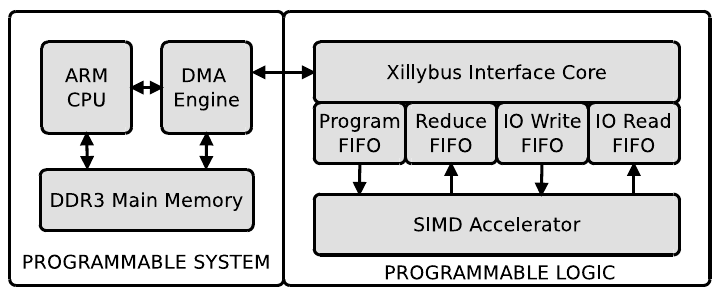
\includegraphics[width=0.6\textwidth]{src/img/connex-arm-arch}
    \caption{Arhitectura Connex-ARM~\cite{opincaa}}
    \label{fig:connex-arm-arch}
\end{figure}

Acceleratorul SIMD utilizat este format din N PEs, iar fiecare dintre acestea
este echipat cu un set de registre interne, o unitate aritmetică logică (ALU), o
logică internă de decodare a instrucțiunilor și o memorie locală (LS). La un
moment de timp, în toate PEs se încarcă aceeași intrucțiune, putând selecta
PEs pe care aceasta să se execute. \\
\abbrev{ALU}{Arithmetic Logical Unit} \abbrev{LS}{Local Storage}

Schimbul de date dintre accelerator și procesorul ARM se face prin trei rețele
corespunzătoare a patru cozi de preluare a datelor, după cum urmează
~\cite{fpga-visual}:
\begin{itemize}
  \item Rețeaua de distribuție, corespunzătoare cozii \code{distributionFIFO},
  este coada prin care instrucțiunile componente ale kernelului sunt distribuite
  către elementele de procesare (PEs) sub forma unui \textit{fully pipelined
  logarithmic tree}.

  \item Rețeaua de I/O \abbrev{I/O}{Input/Output}, corespunzătoare cozilor
  \code{writeFIFO} și \code{readFIFO}, controlează transferul de date de intrare
  și de ieșire dintre memoria principală a procesorului gazdă și memoria locală
  a acceleratorului (\textit{local storage}).

  \item Rețeaua de reducție, corespunzătoare cozii \code{reductionFIFO}, care
  colectează operații globale precum reducerea unei sume, în care se adună toate
  elementele dintr-un anumit registru al elementelor de procesare sub forma unui
  \textit{fully pipelined adder tree}.
\end{itemize}

În mediul de programare OPINCAA, codul pentru accelerator poate fi scris în C++,
utilizând o sintaxă specifică, și se poate intercala cu codul scris pentru GPP.
Se pot folosi date de tip vectorial și operatori caracteristici operațiilor
disponibile pe accelerator, precum reducție, selecție de celule și operații
aritmetice. Codul pentru accelerator este organizat în \textit{kerneluri}, care
sunt compilate și stocate până când se cere lansarea acestora în execuție. \\

În varianta utilizată în această lucrare, sistemul este implementat pe platforma
Xilinx Zynq-7000, care este formată din două componente, identificabile și în
Figura \ref{fig:connex-arm-arch}:
\begin{itemize}
  \item \textbf{Sistemul de procesare} (PS), în care sunt incluse un procesor ARM
  Cortex-A9, care lucrează la o frecvență de \SI{667}{MHz}, un controller de memorie
  DDR SDRAM și un sistem de acces direct la memorie (DMA). \abbrev{PS}{Processing
  System} \abbrev{DDR}{Double Data Rate} \abbrev{SDRAM}{Synchronous Dynamic
  Random-Access Memory} \abbrev{DMA}{Direct Memory Access}

  \item \textbf{Logica programabilă} (PL), alcătuită dintr-un FPGA Artix-7. PL
  se conectează la PS printr-o magistrală de date AMBA AXI, pentru implementarea
  de circuite digitale care să accelereze programele executate de GPP.
  \abbrev{PL}{Programmable Logic}
\end{itemize}

Arhitectura ConnexArray utilizată pune la dispoziție 128 PEs, operanzi pe 16
biți, 32 registre și o memorie locală cu o capacitate de \SI{256}{KB} și consumă, în
medie, \SI{600}{mW}, conform estimărilor efectuate cu programele puse la dispoziție de
Xilinx~\cite{fpga-visual}. Procesorul ARM dual-core consumă, potrivit
documentației Zedboard, maxim \SI{1.25}{W}, ajungând, în medie, la
un total de aproximativ \SI{2}{W} consumați de întregul sistem. \\

\abbrev{SAD}{Sum of Absolute Differences}
\abbrev{SSD}{Sum of Squared Differences}
\abbrev{SIFT}{Scale-Invariant Feature Transform}

Ansamblul format oferă, prin urmare, o opțiune atractivă pentru procesări
dedicate intensive din punct de vedere computațional, cu un consum de putere
redus, fără a sacrifica programabilitatea. În analiza de imagini, de exemplu,
pentru calculul normelor SAD (\textit{sum of absolute differences}) și SSD
(\textit{sum of squared differences}) necesare în algoritmul SIFT
(\textit{scale-invariant feature transform}), s-a obținut un \textit{throughput}
de 4 - 6 ori mai bun folosind acest ansamblu, în comparație cu execuția folosind
doar procesorul ARM, cu un consum de energie de trei ori mai mic, iar în
comparație cu procesoare precum Intel Core i7 2600K sau NVidia GTX680 GPU are un
consum de energie cu până la 40\% mai scăzut.~\cite{fpga-visual}.

\section{Radio definit software}
\label{sec:sdr}

Este considerat un dispozitiv radio, sau, pe scurt, un radio, un dispozitiv care
transmite și recepționează semnale din domeniul radio al spectrului
electromagnetic în scopul transmiterii informației. Un radio definit software,
prescurtat și SDR \abbrev{SDR}{Software Defined Radio}, pornind de la denumirea
în limba engleză Software Defined Radio, este ,,un radio în care o parte
dintre sau toate funcțiile de nivel fizic sunt definite software''
~\cite{sdr-def}. \\

Deși conceptul de SDR era folosit de mai mult timp, până în 1992, odată cu
publicația lui Joseph Mitola despre acest concept în IEEE \cite{mitola-sdr}, nu
exista o viziune unificată asupra sa. Odată cu această publicație,
subiectul a ajuns în atenția unui public mai larg și au fost, totodată, propuse
mai multe direcții de cercetare care au contribuit la consolidarea domeniului. \\

Avantajul implemntării software a funcționalităților de nivel fizic devine
extrem de important în contextul în care tehnologia avansează rapid și se impune
modificarea facilă a dispozitivelor comercializate. În plus, costurile scad
deoarece, în majoritatea cazurilor, nu mai este necesară înlocuirea
echipamentelor, ci doar actualizarea programelor care le descriu funcționarea.
Erorile care pot apărea în anumite echipamente nu mai prezintă un risc major,
deoarece și ele pot fi rezolvate prin actualizarea programului executat de
echipament. Mai mult, odată definite anumite funcționalități, ele pot fi
adaptate pentru mai multe produse, cu modificări minime dependente de platforma
pe care se lucrează. \\

Conceptul a început să ia amploare încă de la sfârșitul anilor '90, când cele
mai multe echipamente de pe piață foloseau un procesor de uz general (GPP)
\abbrev{GPP}{General Purpose Processor} pentru funcții de nivel înalt în rețea
precum interfațarea cu operatorul rețelei sau semnalizare și un procesor de
semnal pentru modulație sau procesare digitală de
semnale~\cite{arslan2007cognitive}. Acest lucru a fost văzut ca o oportunitate
pentru extinderea funcționalității software a echipamentelor, astfel încât s-a
căutat o adaptare mai amplă a lor la schimbările de mediu și la cerințele
utilizatorilor. S-a pus problema unei utilizări mai eficiente și dinamice a
resurselor spectrale, alocarea mai inteligentă a canalelor, precum și relaxarea
constrângerilor legate de interferențe, atunci când este posibil. Astfel, s-au
concretizat domenii precum radio adaptiv, radio cognitiv și radio inteligent,
fiecare o extindere a celui precedent, a căror implementare devine posibilă cu
ajutorul SDR. Figura \ref{fig:sdr-circles} sugerează relația dintre tehnologiile
menționate. \\

\begin{figure}[h]
    \centering
    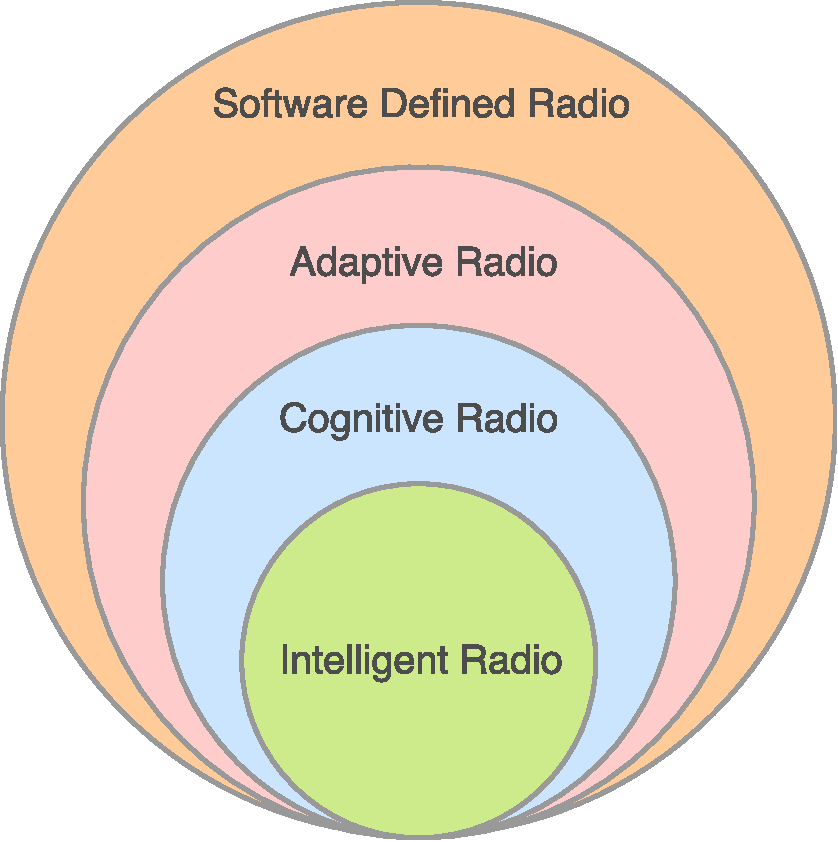
\includegraphics[width=0.5\textwidth]{src/img/sdr-circles}
    \caption{Legătura dintre tehnologiile SDR, AR, CR și IR}
    \label{fig:sdr-circles}
\end{figure}

Deși nu există o definiție unanim acceptată a unui \textbf{radio adaptiv} (AR),
se consideră că acesta este capabil să își monitorizeze performanțele și să
reacționeze la variația acestora prin modificarea parametrilor săi de operare.
În general, el folosește benzi de frecvență nelicențiate care nu sunt
ocupate într-o anumită arie. \abbrev{AR}{Adaptive Radio} \\

Un \textbf{radio cognitiv} (CR) \abbrev{CR}{Cognitive Radio} merge mai departe,
sistemul de comunicații devenind \textit{conștient} de starea lui internă. El va
putea, de exemplu, să recunoască activitățile utilizatorului și să îl asiste în
îndeplinirea acestora, să reacționeze în funcție de locația curentă, recunoscând
servicii disponibile într-o anumită arie. În partea de \textit{backend},
invizibilă pentru utilizator, va putea să optimizeze nivelul rețea folosind
metrici de performanță, să balanseze traficul și va avea un motor care cunoaște
politicile zonelor geografice de operare ale echipamentelor și le respectă în
funcție de cea în care lucrează. De departe, cele mai importante funcționalități
sunt legate de utilizarea spectrului, de aici fiind desprins un domeniul separat
- \textbf{accesul dinamic la spectru} (DSA). \abbrev{DSA}{Dynamic Spectrum
Access} El presupune, printre altele, posibilitatea de a selecta banda de
frecvență în care să lucreze echipamentul pentru a optimiza folosirea resurselor spectrale și
a evita interferențele cu alte echipamente din jurul său. Cu ajutorul acestor
tehnici, va putea să suporte un număr crescut de utilizatori, să fie conștient
de spectrul disponibil, de interferențele și căile de propagare multiple din
jurul său și de puterea semnalului recepțional, utilizând aceste informații
pentru a crește robustețea serviciului~\cite{arslan2007cognitive}.  \\

Un \textbf{radio inteligent} (IR) este deja capabil de învățare automată. El nu numai
că va reacționa în funcție de schimbările mediului, dar va învăța din trecut
pentru a-și îmbunătăți performanțele. \\ \abbrev{IR}{Intelligent Radio}

În concluzie, viitorul sistemelor de comunicații prevede schimbări ambițioase, a
căror limită va fi, în primul rând, puterea de procesare disponibilă pentru
implementarea funcționalităților descrise, care intervine în raportul dintre
costul necesar producerii și întreținerii unui echipament și beneficiile pe care
acesta le aduce. 

% O altă problemă pentru viitor care a
% fost, adesea, neglijată, va fi și densitatea echipamentelor radio și nivelul de
% radiații pe care îl generează. Deși s-a demonstrat că folosirea echipamentelor
% mobile nu crește riscul dezvoltării cancerului la nivelul creierului și a altor
% tumori cerebrale
% ~\cite{us-cancer-institute}\cite{wireless-brain-cancer}\cite{who}, există încă
% incertitudini cu privire la efectul pe termen lung pe care îl pot avea emisiile
% stațiilor de bază~\cite{france-health}.  În acest scop, se poate dovedi utilă
% direcționarea precisă a semnalului ținând cont de poziția utilizatorului, în loc
% de a emite într-un sector întreg. \\

\section{GNU Radio}
\label{sec:gnuradio}

GNU Radio~\cite{gnuradio} este un set de instrumente gratuit și cu sursă deschisă
(\textit{open source}) care facilitează implementarea blocurilor de procesare de
semnal în dispozitivele radio definite software. El pune la dispoziție mai multe
blocuri de procesare clasice, precum filtre, egalizatoare, modulatoare, codoare
etc., și se ocupă de interconectarea blocurilor și schimbul de date dintre ele.
De asemenea, conține și metode pentru definirea unor noi blocuri de procesare
corespunzătoare nevoilor particulare ale dezvoltatorilor. El poate fi folosit
atât pentru a realiza simulări pentru verificarea și stabilirea performanțelor
anumitor blocuri, cât și pentru a se interfața cu dispozitive hardware externe
pentru implementarea propriu-zisă a echipamentelor. \\

Avantajul său major este faptul că dezvoltatorul se poate concentra pe
implementarea blocurilor pentru anumite funcționalități ale echipamentului, fără
a fi nevoie să se ocupe și de comunicația dintre acestea, care este un alt
domeniu în sine, ce necesită un organizator (\textit{scheduler}) eficient ce distribuie
sarcinile blocurilor existente în lanțul de comunicație.  Acest lucru îl face să
lucreze foarte bine atât pe arhitecturi puternice, cu mai multe nuclee, într-un
mod de lucru distribuit, cât și pe procesoare \textit{embedded} unde resursele
de procesare sunt mai limitate. \\

Întrucât algoritmii de localizare a sursei unui semnal sunt folosiți cu
precădere în echipamente de comunicații care se adaptează la mediul
înconjurător, am considerat utilă integrarea kernelurilor pentru accelerarea
algoritmului MUSIC în interiorul GNU Radio, pentru a le asigura disponibilitatea
și refolosirea în mai multe situații. Faptul că implementarea sa software
este disponibilă gratuit și \textit{open source}, îl face ideal pentru
lucrările din mediul academic.  În acest context, este necesară descrierea unor
concepte specifice radiourilor definite software folosite în GNU Radio și a
modului său de lucru. \\

GNU Radio folosește conceptul de lanț de procesare (\textit{flowgraph}) în
organizarea unei aplicații. În acest mod, se face o separare între
funcționalitățile ei, împărțindu-le în blocuri de procesare, care vor fi apoi
interconectate. Fiecare lanț de procesare trebuie să conțină cel puțin o sursă
și un bloc de ,,scurgere'' a semnalului (\textit{sink}). Între aceste două
blocuri are lor procesarea propriu zisă a semnalului. Pentru implementarea lor
este posibilă utilizarea a două limbaje de programare: Python și C++, pentru
acest proiect alegând cea de-a doua variantă, întrucât suntem interesați în
primul rând de performanța modulelor și OPINCAA, mediul de programare pentru
acceleratorul ConnexArray, oferă suport doar pentru acest limbaj de programare. \\

După cum am menționat deja, GNU Radio dispune de o bibliotecă unde sunt deja
implementate o serie de module de uz general. Pentru implementarea unor
funcționalități particulare, se pot defini module proprii, cunoscute și sub
numele de module \textit{out-of-tree} (OOT) \abbrev{OOT}{Out-Of-Tree}, cu
ajutorul utilitarului \code{gr\_modtool}, care va crea o structură de directoare
specifică unui modul GNU Radio. Tot cu ajutorul acestui utilitar se pot adăuga
și noi blocuri în modulul OOT nou creat, specificând anumite caracteristici ale
acestuia: tipul, parametrii de intrare, limbajul folosit etc. \\

La crearea unui bloc, trebuie să analizăm relația dintre intrările și ieșirile
sale, pentru a decide tipul acestuia. Printre tipurile standard de blocuri se
numără \code{general}, \code{sync\_block}, \code{interpolator} și
\code{decimator}.

\begin{itemize}
  \item \code{general} - nu presupune o relație anume între intrări și ieșiri,
  iar o eventuală stabilire a unei legături se poate face prin supraîncărcarea
  funcției \code{forecast}, care este apelată periodic pentru a stabili câte
  date de ieșire se pot produce, reținute în variabila \code{noutput\_items}. În
  mod implicit, relația dintre intrări și ieșiri este de 1:1. În acest caz,
  blocul are o metodă pur virtuală denumită \code{general\_work}, deci care
  trebuie supraîncărcată, în care se va efectua procesarea propriu-zisă din
  bloc. La sfârșitul ei, trebuie specificate câte date de intrare au fost
  consumate și să returnăm numărul de date de ieșire produse.

  \item \code{sync} - un bloc care consumă și produce un număr egal de date pe
  fiecare port. Funcția \code{forecast} este, în acest caz, predefinită și
  metoda în care are loc procesarea poartă denumirea \code{work}. 

  \item \code{source} și \code{sink} - blocuri care au doar ieșiri, respectiv
  doar intrări. 

  \item \code{decimator} și \code{interpolator} - blocuri cu o rată fixă, unde
  numărul de date de intrare este un multiplu al numărului datelor de ieșire,
  respectiv numărul datelor de ieșire este un multiplu al celor de intrare. Pe
  lângă ,,semnătura'' intrărilor și ieșirilor, care reprezintă structurarea lor
  pentru fiecare bloc, acestea primesc ca parametru și factorul de decimare,
  respectiv interpolare.

  \item \code{hierarchical} (bloc ierarhic) - este alcătuit din alte blocuri și,
  la instanțierea acestuia, el se ocupă și de instanțierea blocurilor
  componente.
\end{itemize}

Detaliile specifice implementării blocurilor în GNU Radio vor fi acoperite în
Capitolul \ref{chapter:impl}. \\

O metodă \code{work} este apelată pe baza elementelor de ieșire pe care este capabilă
să le producă la un moment dat, iar \textit{scheduler}-ul GNU Radio gestionează
apelarea acestei metode pe baza cerințelor specifice ale unui bloc, precum
numărul de date de intrare necesare producerii unei date de ieșire, și a stării
\textit{buffer}-elor de intrare sau de ieșire, prin trimiterea de comenzi și
mesaje de stare între blocurile din lanțul de procesare și este cea mai complexă
și remarcabilă parte a întregului sistem~\cite{gnuradio-scheduler}. În plus,
poate aplica restricții legate de alinierea datelor și ajustează pointerii
datelor de intrare și de ieșire, în funcție de cum au fost ,,consumate''. \\

GNU Radio pune la dispoziție și o interfață grafică denumită \textbf{GNU Radio
Companion} cu ajutorul căreia se pot vizualiza blocurile create, precum și cele
deja existente în biblioteci, care se pot asambla într-un lanț de procesare. Cu
ajutorul platformei Qt pentru dezvoltare a elementelor de interfață
grafică, dezvoltatorul își poate crea propriile blocuri cu scopul de a vizualiza
datele obținute. În plus, sunt deja disponibile o serie de astfel de
blocuri, de exemplu pentru vizualizarea spectrului sau a semnalelor în domeniul timp,
asemănător unui osciloscop digital. \\

În concluzie, GNU Radio reprezintă o opțiune atractivă pentru implementarea
eficientă și simplă a blocurilor de procesoare pentru SDR. El beneficiază de o
documentație clară și de o comunitate deschisă, de foarte mare ajutor în
rezolvarea problemelor care pot apărea în dezvoltare.

